\section{Теоретическая часть}

\subsection{Введение}

В качестве осциллятора используется электрический контур, состоящий из последовательно соединенных катушки индуктивности \(L\), конденсатора \(C\), резистора \(R\) и внешнего источника ЭДС (см. \cref{fig:th:1}). 
\begin{figure}[H]
	\centering
	\resizebox{0.4\textwidth}{!}{%
		\begin{tikzpicture}
			% Paths, nodes and wires:
			\draw (7, 4) to[european resistor, l={\normalsize $R$}] (9, 4);
			\draw (9, 2) to[american inductor, l={\normalsize $L$}] (7, 2);
			\draw (7, 4) to[capacitor, l_={\normalsize $C$}, label distance=0.08cm] (7, 2);
			\draw (9, 2) to[rmeter, l_={\normalsize $E(t)$}, label distance=0.08cm] (9, 4);
		\end{tikzpicture}
	}
	\caption{Колебательный контур}
	\label{fig:th:1}
\end{figure}

Целью работы является экспериментальное исследование колебательных процессов в электрическом контуре, состоящем из последовательно соединенных катушки индуктивности \( L \), конденсатора \( C \), резистора \( R \) и внешнего источника ЭДС (см. рис. 1). Такой контур, как и другие системы различной природы, в которых возможны колебания, иногда называют осцилляторами.

Выведем дифференциальное уравнение, описывающее процессы в последовательном колебательном контуре.

Запишем II закон Кирхгофа для нашего контура  
\begin{align} \label{eq:th:1}
	IR + U_C = E(t) + E_i,
\end{align}
где \( I \) — ток в контуре, \( R \) — общее сопротивление контура, \( U_C \) — разность потенциалов между пластинами конденсатора, \( E(t) \) — внешняя ЭДС, а  
\begin{align} \label{eq:th:2}
	E_i = -L \frac{dI}{dt}
\end{align}
-- ЭДС самоиндукции, возникающая на индуктивности.

Заряд \( q \) на обкладках конденсатора связан с напряжением \( U_C \) равенством:  
\begin{align} \label{eq:th:3}
	q = CU_C,
\end{align}

Так как за время \( dt \) заряд конденсатора изменяется на величину  
\( dq = I \cdot dt \), то можно записать:
\begin{align} \label{eq:th:4}
	I = \frac{dq}{dt} = C \frac{dU_c}{dt}
\end{align}

Подставив в уравнение \cref{eq:th:1} значениfя для \( E_i \) из \cref{eq:th:2}, для \( I \) из \cref{eq:th:4} и для \( U_c \) из \cref{eq:th:3}, получим искомое дифференциальное уравнение
\begin{align} \label{eq:th:5}
	L \frac{d^2 q}{dt^2} + R \frac{dq}{dt} + \frac{q}{C} = E(t), 
\end{align}
которое после деления на \( L \) и введения новых обозначений примет  
вид:
\begin{align} \label{eq:th:6}
	\ddot{q} + 2\delta \dot{q} + \omega_0^2 q = f_1(t)
\end{align}

Величина \( \delta = R/2L \) называется коэффициентом затухания,
\begin{align} \label{eq:th:7}
	\omega_0 = \sqrt{\frac{1}{LC}} 
\end{align}
-- собственной частотой контура, а \( f_1(t) = E(t)/L \) -- внешней <<вынуждающей силой>>.

Продифференцировав (6) по \( t \), можно получить аналогичное  
уравнение и для тока в контуре:
\begin{align} \label{eq:th:6a}
	\ddot{I} + 2\delta \dot{I} + \omega_0^2 I = f_2(t), \tag{\ref{eq:th:6}a}
\end{align}

где \( f_2(t) = \dfrac{1}{L} \dfrac{dE}{dt} \) -- <<вынуждающая сила>> колебаний тока.

С математической точки зрения уравнение \cref{eq:th:6} (также как и \cref{eq:th:6a})  
является неоднородным линейным дифференциальным уравнением 2-го порядка с постоянными коэффициентами. Решение такого  
уравнения, как известно, можно представить в виде суммы общего решения соответствующего однородного уравнения:
\begin{align} \label{eq:th:8}
	\ddot{q} + 2\delta \dot{q} + \omega_0^2 q = 0
\end{align} 

и частного решения неоднородного. Уравнение (8) описывает пове-
дение осциллятора в отсутствие внешней ЭДС, т.е. так называемые  
собственные (свободные) колебания, а частное решение неоднородного уравнение \cref{eq:th:6} (в случае периодического внешнего воздействия) -- вынужденные колебания. Исследованию этих двух режимов и уделяется основное внимание в работе. Кроме того, лабораторная установка позволяет наблюдать некоторые переходные процессы, в частности, процессы установления колебаний.

\subsection{Собственные колебания в электрическом контуре}

При анализе решения уравнения  удобно выделить три случая:  
\(\delta < \omega_0\), \(\delta > \omega_0\) и \(\delta = \omega_0\).  

Непосредственной подстановкой в уравнение \cref{eq:th:8} можно убедиться, что в случае достаточно слабого затухания, когда \(\delta < \omega_0\), общее решение уравнения \cref{eq:th:2} можно представить в виде  
\begin{align} \label{eq:th:9}
	q = A_q e^{-\delta t} \cos(\omega_s t + \varphi_q),
\end{align}  
где \(\omega_s = \sqrt{\omega_0^2 - \delta^2}\), \(A_q\) и \(\varphi_q\) --- произвольные постоянные, определяемые из начальных условий. Процесс вида (\ref{eq:th:1}) называют затухающими квазигармоническими колебаниями.  

Аналогичное выражение:  
\begin{align} \label{eq:th:9a}
	I = A_I e^{-\delta t} \cos(\omega_s t + \varphi_I), \tag{\ref{eq:th:9}a}
\end{align}  
--- имеет и зависимость тока в контуре от времени.  

Если \(\delta \ll \omega_0\), то величину \(A(t) = A_q e^{-\delta t}\) можно считать медленно меняющейся амплитудой, а \(T = 2\pi / \omega_s\) --- "периодом" таких колебаний. Качественный график зависимости \(q(t)\) приведен на рис. 2.

В отсутствие затухания (\(\delta = 0\)) амплитуда \(A(t) \equiv const\) и период \(T\) становятся обычными характеристиками гармонического колебания.  

В случае большого затухания (\(\delta > \omega_0\)), решение уравнения \cref{eq:th:8} можно представить в виде:
\begin{align} \label{eq:th:10}
	q = A_1 e^{\alpha_1 t} + A_2 e^{\alpha_2 t},
\end{align}  
где \(A_1\) и \(A_2\) зависят от начальных условий, а
\[\alpha_{1, 2} = - \delta \pm \sqrt{\delta^2 - \omega_0^2}.\]



\begin{figure}[t]
	\centering
	% Первая картинка с меткой и подписью
	\begin{minipage}{0.45\textwidth}
		\centering
		\resizebox{\textwidth}{!}{%
			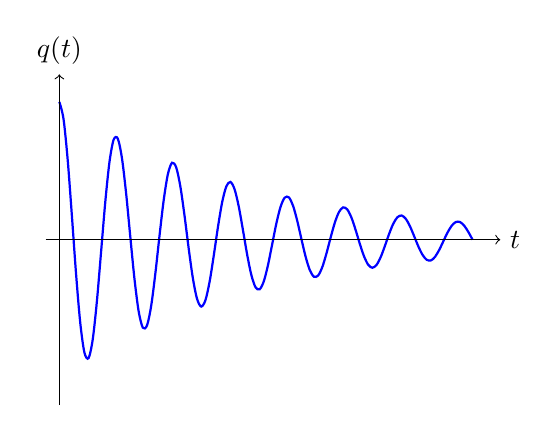
\begin{tikzpicture}[scale=1.75]
				\draw[domain=0.0001:3, samples=100, smooth, blue, thick] 
				plot (\x,{exp(-0.7*\x)*cos(15.19*\x r)});
				
				\draw[->] (-0.1,0) -- (3.2,0) node[right] {$t$};
				\draw[->] (0,-1.2) -- (0,1.2) node[above] {$q(t)$};
			\end{tikzpicture}
		}
		\caption{ }
		\label{fig:2}
	\end{minipage}
	\hfill
	% Вторая картинка с меткой и подписью
	\begin{minipage}{0.45\textwidth}
		\centering
		\resizebox{\textwidth}{!}{%
			\begin{tikzpicture}[scale=1.75]
				\draw[domain=0.0001:3, samples=100, smooth, red, thick] 
				plot (\x,{-(\x / 0.2 - 1) * exp(-(0.31 * \x) / 0.2)});
				
				\draw[->] (-0.1,0) -- (3.2,0) node[right] {$t$};
				\draw[->] (0,-1.2) -- (0,1.2) node[above] {$q(t)$};
			\end{tikzpicture}
		}
		\caption{ }
		\label{fig:3}
	\end{minipage}
	
\end{figure}

Процесс, описываемый формулой \cref{eq:th:9}, называется апериодическим и качественно изображен на \cref{fig:3}.

Условие $\delta = \omega_0$ определяет критический режим колебаний, а соответствующие этому условию сопротивление называется критическим сопротивлением контура: \[R_\text{кр} = 2 \sqrt{\frac{L}{C}}\]

На практике используется также характеристическое (волновое) сопротивление контура:
\[\rho = \sqrt{\frac{L}{C}}\]

\subsubsection{Декремент затухания. Добротность}

Логарифмическим декрементом затухания $d$ называется логарифм отношения значений тока $I$ в контуре в двух последовательных ($n$-ом и $(n+1)$-ом) максимумах:
\begin{align} \label{eq:th:11}
	d = \ln \left(\frac{q_n}{q_{n+1}}\right) = \ln \left(\frac{I_n}{I_{n+1}}\right) = \delta T
\end{align}

Поскольку, как видно из выражений \cref{eq:th:9,eq:th:9a}, $\delta$ есть величина, обратная промежутку времени $\tau$, за которое амплитуда колебаний спадает в $e$ раз, то можно определить число колебаний $N$, совершившихся за это время:
\[N = \frac{\tau}{T} = \frac{1}{\delta T} = \frac{1}{d}\]

Таким образом, логарифмический декремент затухания $d$ есть величина, обратная числу колебаний $N$, в течение которых амплитуда колебаний уменьшается в $e$ раз.

Часто для характеристики затухания удобнее использовать не $N$, а величину в $\pi$ раз большую -- добротность контура $Q = \pi N$.

При малом затухании $(\delta \ll \omega_0)$ частота собственных колебаний \[\omega_S = \sqrt{\omega_0^2 - \delta^2} \approx \omega_0\]

При этом, с использованием выражений для $\omega_0$ и $\delta$, добротность контура и его логарифмический декремент затухания можно выразить через параметры контура $L, C, R$ следующим образом:
\begin{gather}
	\label{eq:th:12} d = \delta T \cong \frac{2\pi}{\omega_0} \delta = \frac{\pi R}{\omega_0 L} = \pi R C \omega_0 = \pi R \sqrt{\frac{C}{L}}, \\
	\label{eq:th:13} Q = \pi N = \frac{\pi}{d} \cong \frac{\omega_0 L}{R} = \frac{1}{RC \omega_0} = \frac{1}{R} \sqrt{\frac{L}{C}}
\end{gather}

Необходимо иметь в виду, что во всех выражениях под $R$ следует понимать сопротивление, эквивалентное всем потерям в контуре. Дополнительные потери при прохождении переменного тока могут быть вызваны гистерезисом и токами Фуко в сердечнике катушки индуктивности, токами утечки и процессами поляризации в диэлектрике конденсатора.

\subsubsection{Фазовая плоскость}

Процессы к колебательном контуре удобно изображать на так называемой фазовой плоскости, где по оси абсцисс откладывают заряд конденсатора $q$, а по оси ординат величину, пропорциональную току, например $q/\omega_0$ (чтобы отложить вдоль осей величины одной размерности и одного порядка величины). Каждому состоянии колебательного контура, характеризуемому мгновенными значениями $q$ и $\dot{q}$, соответствует точка на фазовой плоскости (изображающая точка). Изменение состояния вызывает перемещение изображающей точки по фазовой плоскости. Линия, описываемая изображающей точкой, называется \textbf{фазовой траекторией}. Совокупности движений с разными начальными условиями соответствует семейство фазовых с общим центром в начале координат. Свободные затухающие колебания в контуре (при $\delta < \omega_0$) изображаются фазовыми траекториями в виде скручивающихся к началу координат спиралей, причем скручивание идет тем быстрее, чем больше коэффициент затухания. Апериодическому затухающему процессу соответствуют фазовые траектории, сходящиеся к началу координат. 

\subsection{Вынужденные колебания в электрическом контуре}

Изменение заряда конденсатора под действием внешней гармонической силы в соответствии с \cref{eq:th:6} описывается уравнением:
\begin{align} \label{eq:th:14}
	\ddot{q} + 2 \delta \dot{q} + \omega_0^2 q = F_1 \cos (\omega t),
\end{align}
где $\omega$ -- циклическая частота колебаний вынуждающей силы. Решение уравнения \cref{eq:th:14} и решение аналогично уравнения для тока в контуре, соответствующие установившимся режиму имеют вид: 
\begin{gather}
	\label{eq:th:15} q(t) = q_0 (\omega) \cos (\omega t + \psi_q), \\
	\label{eq:th:15a} \tag{\ref{eq:th:15}a} I(t) = I_0(\omega) \cos (\omega t + \psi_I),
\end{gather}
где $q_0(\omega)$ и $I_0(\omega)$ -- амплитудные значения колебаний заряда на емкости и тока в контуре, а $\psi_q(\omega)$ и $\psi_I(\omega)$ -- имеют смысл фазового сдвига между колебаниями заряда (или тока) и колебаниями внешней ЭДС. Для того, чтобы найти амплитуду и фазу установившихся колебаний воспользуемся методом векторных диаграмм.

\subsubsection*{Метод векторных диаграмм}
\begin{gather}
	\label{eq:th:19} U_L = I_0 \omega L = \frac{\omega L \Epsilon_0}{\sqrt{R^2 + \left(\omega L - \frac{1}{\omega C}\right)^2}}\\
	\label{eq:th:20} U_C = \frac{I_0}{\omega C} = \frac{\Epsilon_0}{\omega C \sqrt{R^2 + \left(\omega L - \frac{1}{\omega C}\right)^2}}\\
	\label{eq:th:21} U_R = I_0 R = \frac{\Epsilon_0 R}{\sqrt{R^2 + \left(\omega L - \frac{1}{\omega C}\right)^2}}
\end{gather}

\subsubsection{Резонансные кривые}

Представим формулы \cref{eq:th:19,eq:th:20,eq:th:21} через переменные $(L, R, C) \to (Q, \omega, \omega_0)
$. Для этого выразим из \cref{eq:th:7,eq:th:13} параметры $Q, \omega_0$:
\begin{align*}
	LC = \frac{1}{\omega^2_0} && \frac{L}{R} = \frac{Q}{\omega_0} && RC = \frac{1}{\omega_0 Q}
\end{align*}

\begin{multline} \label{eq:th:add:1}
	U_L 
	= 
	I_0 \omega L 
	= 
	\frac{\omega \Epsilon_0}{\sqrt{\frac{R^2}{L^2} + \frac{1}{L^2}\left(\omega L - \frac{1}{\omega C}\right)^2}} 
	= 
	\frac{\omega \Epsilon_0}{\sqrt{\frac{R^2}{L^2} + \left(\omega - \frac{1}{\omega LC}\right)^2}}
	=\\=
	\frac{\omega \Epsilon_0}{\sqrt{\frac{\omega_0^2}{Q^2} + \left(\omega - \frac{\omega_0^2}{\omega}\right)^2}}
	=
	\frac{\omega \Epsilon_0}{\sqrt{\frac{\omega_0^2}{Q^2} + \frac{(\omega^2 - \omega_0^2)^2}{\omega^2}}} 
	= 
	\boxed{\frac{\omega^2Q \Epsilon_0}{\sqrt{\omega_0^2 \omega^2 + Q^2 (\omega^2 - \omega_0^2)^2}}}
\end{multline}
\begin{multline} \label{eq:th:add:2}
	U_C 
	= 
	\frac{\Epsilon_0}{\sqrt{\omega^2 C^2 R^2 + \left(\omega^2 LC - 1\right)^2}}
	=
	\frac{\Epsilon_0}{\sqrt{\frac{\omega^2}{\omega_0^2 Q^2} + \left(\frac{\omega^2}{\omega_0^2} - 1\right)^2}}
	=\\=
	\boxed{\frac{\omega_0^2 Q \Epsilon_0}{\sqrt{\omega^2 \omega_0^2 + Q^2 (\omega^2 - \omega_0^2)^2}}}
\end{multline}
\begin{multline} \label{eq:th:add:3}
	U_R 
	= 
	\frac{\Epsilon_0}{\sqrt{1 + \frac{1}{R^2}\left(\omega L - \frac{1}{\omega C}\right)^2}}
	=
	\frac{\Epsilon_0}{\sqrt{1 + \left(\omega \frac{L}{R} - \frac{1}{\omega RC}\right)^2}}
	=
	\frac{\Epsilon_0}{\sqrt{1 + \left(\frac{\omega Q}{\omega_0} - \frac{\omega_0 Q}{\omega }\right)^2}}
	=\\=
	\frac{\Epsilon_0}{\sqrt{1 + Q^2\frac{(\omega^2 - \omega_0^2)^2}{\omega^2 \omega_0^2}}}
	=
	\boxed{\frac{ \omega \omega_0 \Epsilon_0}{\sqrt{\omega^2 \omega_0^2 + Q^2 (\omega^2 - \omega_0^2)^2}}}
\end{multline}

Для нахождения максимумов функций найдем производные \cref{eq:th:add:1,eq:th:add:2,eq:th:add:3}:
\begin{multline*}
	(U_L)_\omega' 
	= 
	Q \Epsilon_0 \frac{2 \omega \sqrt{\omega_0^2 \omega^2 + Q^2 (\omega^2 - \omega_0^2)^2} - \omega^2 \left(\sqrt{\omega_0^2 \omega^2 + Q^2 (\omega^2 - \omega_0^2)^2}\right)'_\omega}{\omega_0^2 \omega^2 + Q^2 (\omega^2 - \omega_0^2)^2}
	=\\=
	Q \Epsilon_0 \frac{2 \omega \sqrt{\omega_0^2 \omega^2 + Q^2 (\omega^2 - \omega_0^2)^2} - \omega^2 \dfrac{2\omega\omega_0^2 + 4 \omega Q^2(\omega^2 - \omega_0^2)}{2\sqrt{\omega_0^2 \omega^2 + Q^2 (\omega^2 - \omega_0^2)^2}}}{\omega_0^2 \omega^2 + Q^2 (\omega^2 - \omega_0^2)^2}
	=\\=
	Q \Epsilon_0 \frac{4 \omega \big(\omega_0^2 \omega^2 + Q^2 (\omega^2 - \omega_0^2)^2\big) - \omega^2 \left(2\omega\omega_0^2 + 4 \omega Q^2(\omega^2 - \omega_0^2)\right)}{\left(\omega_0^2 \omega^2 + Q^2 (\omega^2 - \omega_0^2)^2\right)^{3/2}}
	=\\=
	Q \Epsilon_0 \frac{4 \omega_0^2 \omega^3 + 4 \omega Q^2 (\omega^2 - \omega_0^2)^2 - 2\omega^3\omega_0^2 - 4 \omega^3 Q^2(\omega^2 - \omega_0^2)}{\left(\omega_0^2 \omega^2 + Q^2 (\omega^2 - \omega_0^2)^2\right)^{3/2}}
	=
	0
\end{multline*}
\[2 \omega_0^2\omega^3 - 4 \omega \omega_0^2 Q^2 (\omega^2 - \omega_0^2) = 0\]
\[2 \omega_0^2 \omega \left( \omega^2 - 2Q^2 (\omega^2 - \omega_0^2) \right) = 0\]
\[\omega^2(1 - 2 Q^2) = - 2 \omega_0^2 Q^2\]
\begin{align} \label{eq:th:add:5}
	\boxed{\omega_L = \frac{\omega_0}{\sqrt{1 - \dfrac{1}{2Q^2}}}}
\end{align}

\[(U_C)_\omega' 
= 
\omega_0^2 Q \Epsilon_0 \cdot\left(\sqrt{\omega^2 \omega_0^2 + Q^2 (\omega^2 - \omega_0^2)^2}\right)'_\omega 
= 
\omega_0^2 Q \Epsilon_0 \cdot \frac{2 \omega_0^2 \omega + 4\omega Q^2(\omega^2 - \omega_0^2) }{2 \sqrt{\omega^2 \omega_0^2 + Q^2 (\omega^2 - \omega_0^2)^2}}\]
\[2 \omega_0^2\omega + 4 \omega^3 Q^2 - 4 \omega \omega_0^2 Q^2 = 0\]
\[\omega(2 \omega^2_0 + 4 \omega^2 Q^2 - 4 \omega_0^2 Q^2) = 0\]
\[4 \omega^2 Q^2 = 4 \omega_0^2 Q^2 - 2\omega_0^2\]
\begin{align} \label{eq:th:add:4}
	\boxed{\omega_C = \omega_0\sqrt{1 - \frac{1}{2Q^2}}}
\end{align}

\begin{multline*}
	(U_R)_\omega' 
	=
	\omega_0 \Epsilon_0 \frac{
		\sqrt{\omega^2 \omega_0^2 + Q^2 (\omega^2 - \omega_0^2)^2} - \omega \left( \sqrt{\omega^2 \omega_0^2 + Q^2 (\omega^2 - \omega_0^2)^2}  \right)'_\omega
	}{
		\omega^2 \omega_0^2 + Q^2 (\omega^2 - \omega_0^2)^2
	}
	=\\=
	\frac{2\omega^2 \omega_0^2 + 2Q^2 (\omega^2 - \omega_0^2)^2 - \omega \left(2 \omega \omega_0^2 + 4\omega Q^2(\omega^2 - \omega_0^2)\right)}{\left(\omega^2 \omega_0^2 + Q^2 (\omega^2 - \omega_0^2)^2\right)^{3/2}}
	=\\=
	\frac{
		2\omega^2 \omega_0^2 + 2Q^2 (\omega^2 - \omega_0^2)^2 - 2 \omega^2 \omega_0^2 - 4 \omega^2Q^2 (\omega^2 - \omega_0^2)
	}
	{
		\left(\omega^2 \omega_0^2 + Q^2 (\omega^2 - \omega_0^2)^2\right)^{3/2}
	}
	=\\=
	\frac{
		2Q^2 (\omega^2 - \omega_0^2)^2  - 4 \omega^2Q^2 (\omega^2 - \omega_0^2)
	}
	{
		\left(\omega^2 \omega_0^2 + Q^2 (\omega^2 - \omega_0^2)^2\right)^{3/2}
	}
	=
	0
\end{multline*}
\[(\omega^2 - \omega_0^2)(2\omega^2 Q^2- 2\omega_0^2Q^2 - 4 \omega^2 Q^2) = 0\]
\[2 \omega^2 Q^2 = 2 \omega_0^2Q^2 \]
\begin{align} \label{eq:th:add:6}
	\boxed{\omega_R = \omega_0}
\end{align}

Подставим значения \cref{eq:th:add:4,eq:th:add:5,eq:th:add:6} в \cref{eq:th:add:1,eq:th:add:2,eq:th:add:3}, получим:
\begin{align}
	U_C^{max} = \frac{\Epsilon_0 Q}{\sqrt{1 - \frac{1}{4Q^2}}} &\text{, при } \omega_c^{max} = \omega_0 \sqrt{1 - \frac{1}{2Q^2}}\\
	U_L^{max} = \frac{\Epsilon_0 Q}{\sqrt{1 - \frac{1}{2Q^2}}} &\text{, при } \omega_L^{max} = \frac{\omega_0}{\sqrt{1 - \dfrac{1}{2Q^2}}}\\
	U_R^{max} = \Epsilon_0 &\text{, при } \omega_R^{max} = \omega_0
\end{align}
